\documentclass[a4paper,12pt]{article}

\usepackage[utf8]{inputenc}
\usepackage[T1]{fontenc}
\usepackage[french]{babel}
\usepackage{graphicx}
\graphicspath{{./Images/}}
\usepackage{xcolor}
\usepackage{amsmath, amssymb}
\usepackage[left=3cm,right=3cm,top=2cm,bottom=2cm]{geometry}
\usepackage{listings}
\usepackage[vlined, lined, linesnumbered, boxed, french]{algorithm2e}

\begin{document}

\begin{figure}
    \centering
    
\includegraphics[width=0.5\textwidth]{enseirb-matmeca.png}
\end{figure}

\begin{center}
\vspace{0.5\baselineskip}
  \Huge
  { \huge \bfseries HEX}\\[0.4cm]
\vspace{\baselineskip}
\large
\begin{center}
 \rule{0.5\linewidth}{1pt}
 \end{center}
 
Projet réalisé par \\
\large
\vspace{1\baselineskip}
Boullit Mohamed Fayçal\\
Izekki Jalal\\
Moussa Guimba Mamadou\\
Pierre Hugo\\
\begin{center}
 \rule{0.5\linewidth}{1pt}
 \end{center}
\vspace{2\baselineskip}
\large
Projet encadré par \\
\vspace{1\baselineskip}
Herbreteau Frédéric\\
\large
\vspace{3\baselineskip}
Equipe 9151\\
\vspace{3\baselineskip}
Année 2019/2020
\end{center}
\newpage

\tableofcontents
\newpage


\section{Introduction}
Dans le cadre du second projet de première année, filière informatique, il nous est proposé de mettre en application nos compétences en programmation en implémentant le jeu Hex, écrit en langage C.\\
Hex est un jeu de société opposant deux joueurs, qui se joue sur un tablier formé par des hexagones réguliers. Les joueurs sont représentés chacun par une couleur et possèdent des pions de leur couleur qu'ils disposent un à un sur les cases vides de leur choix du plateau. L'objectif de tout joueur est de réussir à construire un chemin continue de pions reliant les deux bords de sa couleur.\\
Nous allons vous faire découvrir en profondeur le jeu de Hex dans ce projet et les différentes stratégies de jeu permettant de remporter la partie. Pour ce faire nous allons mettre en place un ensemble de clients possédant une interface commune mais qui ont leur propre plateau de jeu et jouant en fonction de leur propre stratégie et un serveur qui permet l'interaction entre deux clients.


\begin{figure}[h]
    \centering
    \label{fig:Hexgraph}
    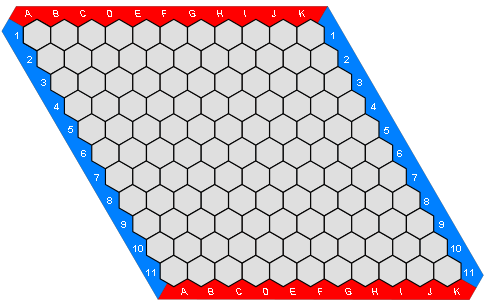
\includegraphics[width=0.3\textwidth]{Images/Hex.png}

    \caption{Tablier du jeu vide}
\end{figure}
\section{Le plateau de Jeu}

\subsection{Représentation du plateau}
\label{sec:plateau_de_jeu}
Le plateau de jeu est représenté par un graphe dont les noeuds sont exactement les cases du palier. Pour manipuler le graphe, la bibliothéque GSL (GNU Scientific Library) est utilisée. C'est une bibliothéque numérique pour les programmeurs C et C ++ qui fournit dans le cadre de ce projet des fonctions qui manipulent des matrices creuses. Ce qui permet de modéliser le graphe en considérant une matrice d'adjacence t de taille $n\times n $ qui vérifie la propriété t[i][j] = 1 si et seulement s'il existe une arrête entre le noeud i et le noeud j où n est le nombre de sommet du graphe. Une autre matrice o est définie de taille $2\times n$ qui vérifie que o[k][i] = 1 si et seulement si le noeud i est occupé par le joueur k.
Plus précisément, une structure nommé \textbf{graph\_t} représente le graphe. Elle est constituée du nombre total de noeud et des deux matrices creuses citées précédemment:
\begin{lstlisting}[language={C},captionpos=b, frame=single]
    struct graph_t {
  size_t num_vertices;  // Number of vertices in the 
  gsl_spmatrix* t;  
  gsl_spmatrix* o;      
};
\end{lstlisting}
Dans ce projet, nous travaillons avec trois types de graphe de taille variable à savoir le graphe hexagonal, carré et triangulaire représentés sur la figure suivante.
\begin{figure}[h]
    \centering
    \label{fig:Hexgraph}
    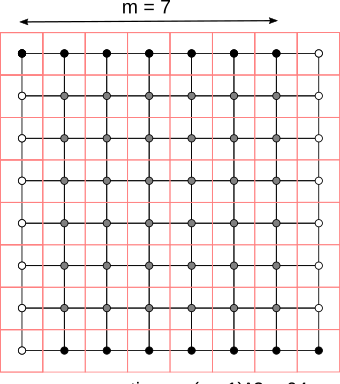
\includegraphics[width=0.3\textwidth]{Images/carre.png}
    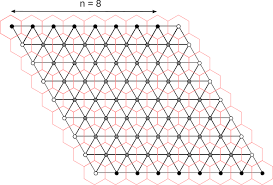
\includegraphics[width=0.5\textwidth]{Images/hexagonal.png}
    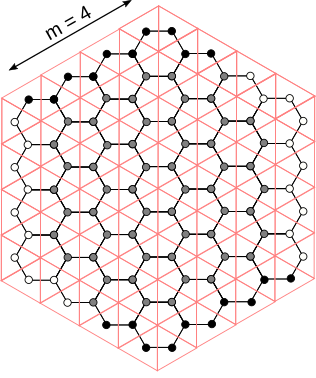
\includegraphics[width=0.3\textwidth]{Images/triangulaire.png}
    \caption{Les types de graphe utilisés}
\end{figure}

\subsection{Les coups de jeu}

Nous représentons un coup de jeu par une structure \textbf{struct move\_t} qui contient le numéro du noeud choisi par le joueur ainsi que la couleur du joueur. 
\begin{lstlisting}[language={C},captionpos=b, frame=single]
    struct move_t {
    size_t m; 
    enum color_t c;
\end{lstlisting}

On choisi les couleurs: BLACK = 0 et WHITE = 1 pour désigner les joueurs. Le joueur de couleur Noir est celui qui commence la partie de jeu.  

\subsection{Les coups de jeu}

\section{Mise en oeuvre technique}


\subsection{Les joueurs}
\label{sec:joueurs}

Les différents joueurs sont codés indépendamment et sont sauvegardés dans des bibliothèques dynamiques qui pourront être chargées dynamiquement par le serveur.
Afin de définir l'inter-fonctionnalité entre les différents clients, une même interface est requise pour tous les joueurs.\\
Tout joueur doit sauvegarder le graphe que lui passe le serveur et doit être capable de proposer et d'accepter ou non un coup en fonction de la situation dans laquelle il se trouve. C'est ce que font respectivement les fonctions \textbf{initialize\_graph}, \textbf{propose\_opening} et \textbf{accept\_opening}. Vient alors la fonction \textbf{initialize\_color} qui assigne à chaque joueur sa couleur et la fonction \textbf{play} qui permet au joueur de proposer son coup en fonction de sa stratégie.

\subsection{Le serveur}

Le serveur est le programme qui permet le déroulé du jeu, en envoyant les informations aux stratégies et en vérifiant l'avancement de la partie.

\subsubsection{La boucle de jeu}

La boucle de jeu est toute simple, dans un premier temps une copie du graphe représentant le plateau de jeu est envoyé à chacun des joueurs, ce ne sont que des copies afin d'éviter toute triche qui consisterait à modifier le plateau de jeu en changeant par exemple des cases déjà colorées.\\

Le démarrage de la partie se fait selon la règle dit du gâteau, elle consiste à demander à un joueur de jouer un premier coup, puis de demander au second joueur si il veut prendre ce coup pour lui ou le laisser à l'autre joueur, le serveur attribue ainsi leur couleur à chaque joueur, le joueur ayant le premier coup est le joueur noir.\\

Vient ensuite la boucle de jeu à proprement parler, cette dernière consiste en une boucle tant que vérifiant que le graphe n'est pas entièrement coloré. À chaque tour le serveur calcule le prochain joueur puis lui fait jouer son coup et enfin fait appel à la fonction \textbf{is\_winning} vérifie si la partie est terminée. Cette fonction renvoie un booléen indiquant si la partie est terminé ce qui de stopper la boucle à l'aide d'un \textbf{break}.\\

\begin{algorithm}[H]

G $\leftarrow$ graph\_\_initialize(M, T);\\
\For{ tout joueur p }{
    p->initialize\_\_graph(G)}
move = joeur1->propose\_opening();\\   
\eIf{joeur2->accept\_opening(move)}{
    C'est le joeur2 qui joue le prochain coup donc\\
    joueur1->initialize\_color(BLACK);\\
    joueur2->initialize\_color(WHITE);}{
    C'est le joeur1 qui joue encore une fois et donc\\
    joueur1->initialize\_color(WHITE)\\
    joueur2->initialize\_color(BLACK);}
\While{G n'est pas rempli}{
    p $\leftarrow$ le joueur suivant;\\
    move = p->play(move);\\
    \eIf{Il gagne avec le noeud \textbf{move}}
    {\textbf{break}}{}}

\caption{Principe algorithmique de la boucle de jeu}
\end{algorithm}

\subsubsection{La fonction \textbf{is\_winning}}
Cette fonction est celle permettant au serveur de savoir si la partie est terminée, mais elle est également celle qui colore le graphe pour le serveur. Pour ce faire, elle prend en paramètre un pointeur vers une structure \textbf{struct game} qui réunie le plateau de jeu ainsi que les joueurs représentés par la structure \textbf{struct player} (voir section \ref{sec:com_joueurs}), le coup jouer représenté par la structure \textbf{struct move}, ainsi qu'un caractère indiquant la forme du plateau de jeu (voir section \ref{sec:plateau_de_jeu}) et la taille du graphe.

Dans un premier temps, la fonction vérifie si le coup est possible et si oui colore le graphe en fonction.

Vient alors la vérification pour savoir si le dernier joueur ayant jouer a gagné la partie. Cela se fait par un parcours en profondeur sur le sous-graphe de la couleur de ce joueur afin de repérer une éventuelle connexion entre les deux partie colorées d'origines du joueur. Pour ce faire, il y a deux fonctions qui calculent les indices d'un nœuds dans une partie et dans l'autre, pour cela elles prennent en paramètre la forme du graphe, sa taille ainsi que la couleur testée. Le premier nœud sert de départ pour le parcours en profondeur et si le deuxième nœud est rencontré lors de ce parcours alors les deux parties sont reliées et le joueur à gagner.

\subsubsection{Communication avec les joueurs}
\label{sec:com_joueurs}

Comme vu dans la section \ref{sec:joueurs}, les joueurs sont codés dans des bibliothèques appelées dynamiquement. Cet appel est réalisé grâce à la bibliothèque \textbf{dlfcn} qui permet d'ouvrir dynamiquement une bibliothèque. Les stratégies sont donc données en paramètre lors du lancement du serveur.

Une structure \textbf{struct player} réunie les pointeurs des fonctions fournies par la bibliothèque du joueur (partie \ref{joueurs}) ainsi que le pointeur vers cette bibliothèque pour pouvoir la fermer à la fin de la partie.

\subsection{Implémentation des graphes}
La structure \textbf{graph\_t} évoquée dans la partie \ref{sec:plateau_de_jeu}, nécessite plusieurs fonctions pour la manipuler, et parmi les fonctions principales on trouve \textbf{graph\_initialize} une fonction qui prend en paramètre la longueur du tablier souhaité, et la forme (hexagonal,carré ou triangulaire) et qui retourne un pointeur vers une structure \textbf{graph\_t} allouée et bien initialisée. La seconde fonction qui réside importante c'est la fonction qui permet au serveur de créer des copies pour les joueurs \textbf{graph\_copy}, ainsi qu'une liste de fonction qui ne laisse plus le besoin de faire appel à une fonction de la bibliothèque GSL en dehors du fichier \textit{graph\_function.c}.
Le tablier est affiché par la fonction \textbf{graph\_print} qui prend le graphe en paramètre, et sa forme pour l'afficher correctement.
\section{Les différentes stratégies de jeu}


\subsection{La stratégie aléatoire}
La stratégie aléatoire consiste à proposer un coup objectivement parmi les coups possibles. S'il arrive qu'il débute la partie, le coup qu'il propose est également aléatoire sinon, il accepte toujours le coup joué par l'adversaire.
Ainsi, le principe algorithmique sur lequel repose la stratégie aléatoire est le suivant: 
\\

\begin{algorithm}[H]
 \KwData{Le dernier coup \textbf{pm} du joueur adverse}
 \KwResult{Le coup \textbf{nm} du joeur aléatoire}

marquer dans le graphe le coup du joueur adverse;\\    
choisir aléatoirement un noeud \textbf{nm} quelconque du plateau jeu\\
\While{le noeud \textbf{nm} est occupé}{
    choisir aléatoirement un autre noeud \textbf{nm} \\
    }
colorer dans le graphe le noeud choisi;\\
retourner le noeud

\caption{Principe algorithmique du coup aléatoire}
\label{algoAléatoire}
\end{algorithm}

\subsection{La stratégie du bloqueur}

Le joueur qui utilise cette stratégie de jeu a pour but de bloquer les coups de son adversaire. En effet, comme l'adversaire essaye de joindre les deux bords du plateau correspondant à sa couleur par un chemin continue, l'objectif du bloqueur est de mettre un obstacle devant chacun de ses coups joués.
Cependant le choix des noeuds à occuper dépend de la couleur avec la quelle joue le client stratège.
Considérons par exemple un graphe hexagonale comme schématisé sur la figure 3:
\begin{itemize}
    \item Si le bleu représente l'adversaire, bloquer son coup revient à choisir l'un des noeuds blancs(C'est celui de gauche qui est généralement choisit). S'il arrive qu'ils soient occupés, le joueur rouge choisit un parmi les noeuds marrons mais généralement c'est le premier à gauche qui est choisit.
    
    \item Par contre si le rouge représente l'adversaire, la stratégie est de privilégier les noeuds marrons aux noeuds blancs.
\end{itemize}
S'il s'avère que tous les voisins du coup joué par l'adversaire sont colorés, le joueur propose aléatoirement un coup parmi ceux possibles.
\begin{figure}[h]
    \centering
    \label{fig:coupbloqueur}
    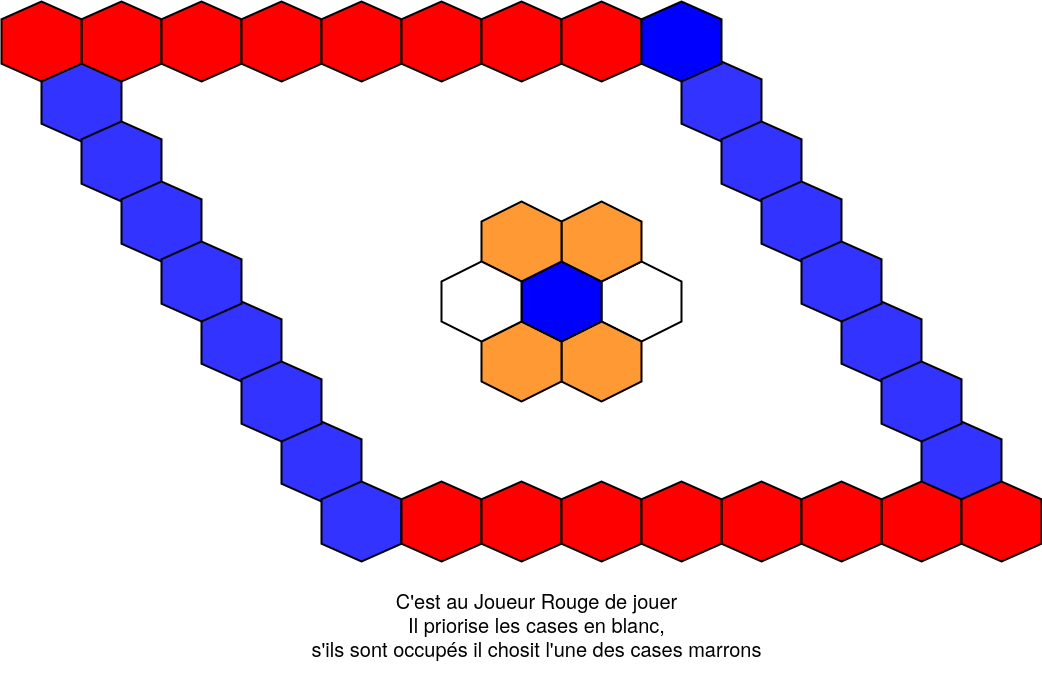
\includegraphics[width=0.4\textwidth]{Images/rouge.png}
    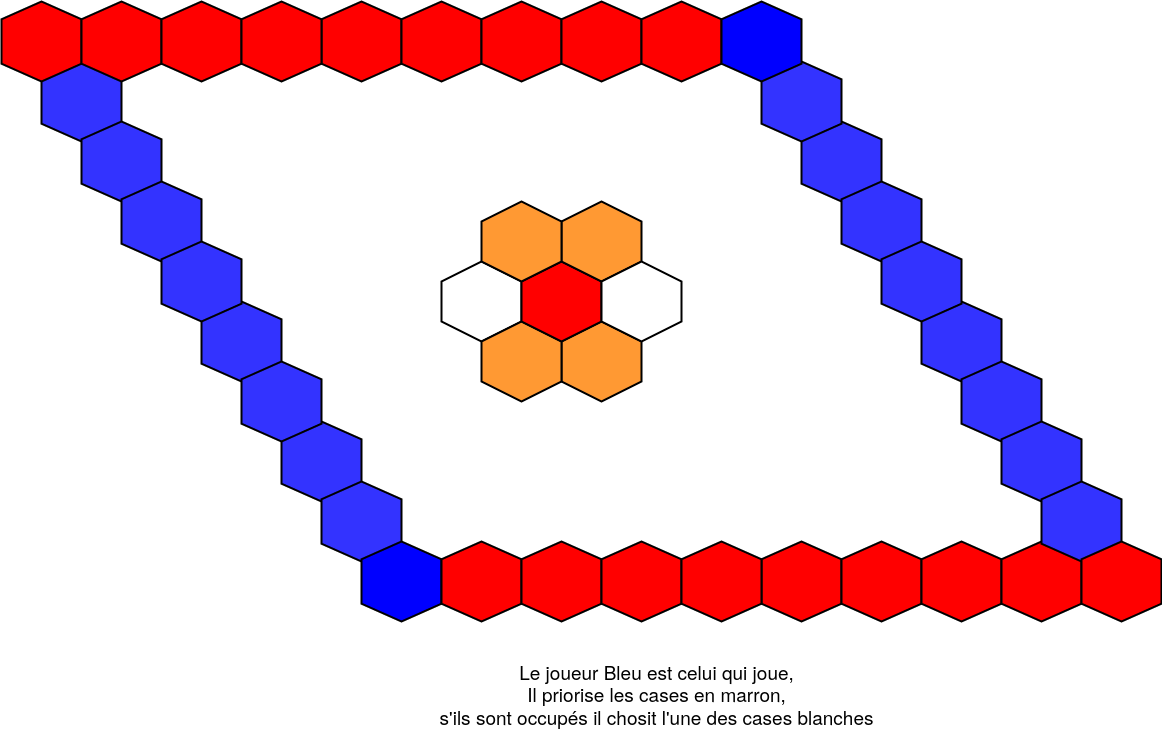
\includegraphics[width=0.4\textwidth]{Images/bleue.png}
    \caption{Choix du noeud obstacle}
\end{figure}

Ainsi, le principe algorithmique sur lequel repose cette stratégie est le suivant:
\begin{algorithm}[H]
 \KwData{Le dernier coup \textbf{pm} du joueur adverse}
 \KwResult{Le coup \textbf{nm} du joeur aléatoire}

marquer dans le graphe le coup \textbf{pm} joué par l'adversaire;\\   
Soit T un ensemble vide;\\
T $\leftarrow$ tous les noeuds inoccupés qui sont voisins à \textbf{pm};\\
\eIf{T n'est pas vide}{
    \eIf{Le joueur qui joue est le rouge}{
    privilégier le noeud de gauche et celui de droite du noeud rouge;\\
    s'ils sont colorés choisir un noeud non coloré parmi les quatre autres;\\}{
    privilégier les noeuds placés au dessus et en dessous du noeud bleu;\\
    s'ils sont tous occupés, choisir soit celui de gauche ou celui de droite;\\}}
    {
    choisir aléatoirement un noeud inoccupée}
colorer dans le graphe le noeud choisi;\\
retourner le noeud

\caption{Principe algorithmique de la stratégie du bloqueur}
\label{algoBi}
\end{algorithm}

\subsection{la stratégie du coup maintenant le plus court chemin}
Cette stratégie se base essentiellement sur le maintien du plus court chemin après chaque coup joué par l'adversaire. En effet une structure stratégie est nécessaire pour stocker les indices des bords du plateau au début du jeu qui permettront de déterminer à chaque fois le chemin le plus court à travers le fameux algorithme \textit{DIJSKTRA}. A chaque fois qu'un chemin est généré on suppose que $n$ est la distance ou bien le nombre de cases restantes pour ce chemin, à ce stade pour trouver le prochain coup, on colore chaque case du chemin par la couleur de l'adversaire si jamais on ne trouve pas un chemin alternative de profondeur n, donc cette case colorée est la seule à avoir maintenu la notion du plus court chemin, c'est bien la case à jouer.

\begin{figure}[h]
    \centering
    \label{fig:Hexmove}
    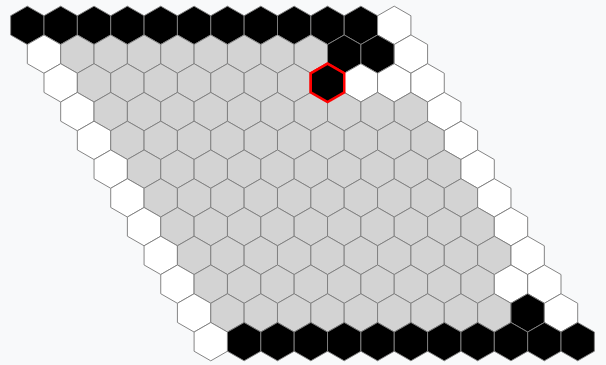
\includegraphics[width=0.85\textwidth]{Images/Hex_move_shortest.png}

    \caption{Prochain coup généré par l'algorithme pour le joueur noir}
\end{figure}

La figure \ref{fig:Hexmove} montre le coup choisi par l'algorithme, avant de jouer le coup choisi entouré en rouge, le plus court chemin était de profondeur 9, et ce coup étant un parmi les coups minimisants la profondeur du plus court chemin, mais étant le seul à avoir garder plus de 2 chemins de profondeur 8 par suite, en supposant n'importe quel prochain coup de l'adversaire dans le cas de la figure \ref{fig:Hexmove} le joueur garde toujours un second chemin de profondeur 8 à suivre.\\

\begin{algorithm}[H]
 \KwData{Tablier du jeu \textbf{T}, Couleur du joueur \textbf{c}}
 \KwResult{Le coup \textbf{n}}

$Chemin \leftarrow$ plus court chemin entre les deux bords colorés en \textbf{c} de \textbf{T};\\
$profondeur \leftarrow$ $taille(chemin)$; \\    
\If{$Chemin\ est\ vide$}{
    $n \leftarrow$ coup aléatoire valide ;
}
\While{$Chemin\ ! vide$}{
    $n \leftarrow$ noeud du Chemin;\\
    Retirer $n$ du Chemin;\\
    Colorer le noeud $n$ par la couleur inverse de \textbf{c};\\
    $alternative \leftarrow$ plus court chemin entre les deux bords;\\
    \If{$profondeur < taille(alternative)$}{
        \textbf{break}
        \\}}
colorer dans le graphe $n$ choisi par la couleur \textbf{c};\\
retourner n;

\caption{Principe algorithmique du coup maintenant le plus court chemin}
\label{algoShortPath}
\end{algorithm}
La complexité de l'algorithme est \textbf{quadratique} en nombre de sommets, dû à celle de \textit{Dijsktra} implémenté en utilisant des tableaux. Ce qui demande un temps raisonnable au joueur pour répondre au coup de l'adversaire.

\subsection{la stratégie "two-distances"}
La stratégie implémenté basée sur le principe du deux-distances \textit{(two-distances, van Rijswijck, 2000)} est fournit principalement par l'algorithme \textit{Minimax}. En effet,\textit{two-distances} est une façon d'évaluer un tablier. En l'évaluant, on peut déterminer le joueur qui est susceptible de gagner. Le problème avec la stratégie précédente c'est que si l'adversaire bloque le joueur un peu plus loin, le joueur n'a aucune information sur l'existence de son plus court chemin et du chemin alternatif, d'où l'idée d'évaluer plus de positions.
\subsubsection{Méthode de Minimax}
La stratégie minimax détermine les valeurs des positions du tablier non terminales ou détermine de nouvelles positions terminaux. L'algorithme suppose un jeu optimal alternatif des deux côtés et recherche les branches de l'arbre vers les nœuds terminaux, ou  jusqu'à une profondeur donnée. Dans le cas du jeu de Hex la taille du tablier ne permet pas d'aller jusqu'au bords, d'où la nécessité d'une fonction qui évalue un tablier avec quelques coups. 
\subsubsection{Évaluation "two-distances"}
La fonction d'évaluation \textit{two-distances} est basée sur la mesure de la connectivité relative d'une position Hex, et qui prend en considération la présence des chemin alternatifs. Son principe définit la distance $d(u,v)$ pour deux sommets $u$ et $v$ comme suit:
\begin{equation}
    d(u,v) = 1\ ,\ Si\ u\ et\ v\ sont\ voisins. \\
\end{equation}
Sinon, en supposant $N(u)$ l'ensemble des voisins de $u$, et en retirant $u'$ le voisin de $u$ de plus proche distance de v, on considère un nouveau voisin $u'' \in N(u)$ le plus proche de v, et on définit:
\begin{equation}
    d(u,v) = 1 + d(u'',v)
\end{equation}
Alors, en considérant $e_{1p}$ $e_{2p}$ deux sommets appartenant respectivement aux deux bords du tablier de la même couleur pour un joueur $p$, la fonction d'évaluation du tableau $f$ est la distance entre les deux sommets: \\
\begin{equation}
    f(p) = d(e_{1p},e_{2p})
\end{equation}

\subsubsection{Principe implémenté}
Le principe implémenté et décrit par l'algorithme \ref{algominimax} consiste à minimiser la distance entre les deux bords du tablier du joueur en jouant un coup. Par l'algorithme de \textit{minimax}, on souhaite évaluer les noeuds du tablier, l'évaluation d'un noeud dans un tablier vide de forme hexagonale coûte $\mathcal{O} (6^{d}\times c) $, où $c$ est la complexité de la fonction d'évaluation, $d$ la profondeur souhaitée lors de l'utilisation de \textit{mimimax}. En effet, une grande complexité résulte de la fonction d'évaluation où on utilise \textit{DIJSKTRA} pour trouver les voisins $u'$ et $u"$ ce qui rend l'algorithme plus complexe.\\
Alors, afin de minimiser le temps de calcul du joueur, un choix optimal des noeuds évalués est fait, il consiste à ne prendre en considération que l'ensemble des noeuds définissant l'intersection des plus courts chemins pour chaque joueur.\\ \\
\begin{algorithm}[H]
 \KwData{Tablier du jeu \textbf{T}, Couleur du joueur \textbf{c}, Profondeur \textbf{p}, Fonction d'évaluation \textbf{f}}
 \KwResult{Le coup \textbf{n}}

$Chemin1 \leftarrow$ plus court chemin entre les deux bords colorés en \textbf{c} de \textbf{T};\\
$Chemin2 \leftarrow$ plus court chemin entre les deux bords colorés en \textbf{{c}} de \textbf{T};\\
$Region \leftarrow Chemin1 \cap Chemin2 $; \\    
\eIf{$Region\ est\ vide$}{
    $n \leftarrow$ coup aléatoire valide ;
}{
$n \leftarrow Minimax(T,p,-\infty,+\infty,Region,Minimisation,f)$
}
colorer dans le graphe $n$ choisi par la couleur \textbf{c};\\
retourner \textbf{n};

\caption{Principe algorithmique du coup évalué par Minimax à travers l'évaluation $f$}
\label{algominimax}
\end{algorithm}


La fonction \textit{Minimax} utilisée est optimisée par l'élagage alpha-Beta, ce sont les deux paramètres initialisés lors de l'appel de \textit{Minimax} en $+\infty$ et $-\infty$, le paramètre $Minimisation$ est un booléen indiquant le souhait de la minimisation de la distance entre les deux bords pour ce joueur, $p$ c'est la profondeur du calcul.

\section{Conclusion}

Ce projet avait pour objectif l'implémentation d'un serveur organisant une partie du jeu de Hex entre deux clients. Partant d'une stratégie aléatoire, plusieurs autres stratégies ont étés implémentés dont les plus efficaces sont la stratégie du coup maintenant le plus court chemin et celle des "two-distances".\\
Ce projet nous a ainsi permis d'approfondir nos connaissances en programmation impérative comme l'utilisation des bibliothèques dynamiques ainsi que leur chargement mais aussi de mettre en application des notions de théorie des graphes comme le parcours en profondeur et le problème du plus court chemin.





\end{document}